\documentclass{standalone}
\usepackage{tikz}
\usetikzlibrary{patterns, positioning}


\begin{document}
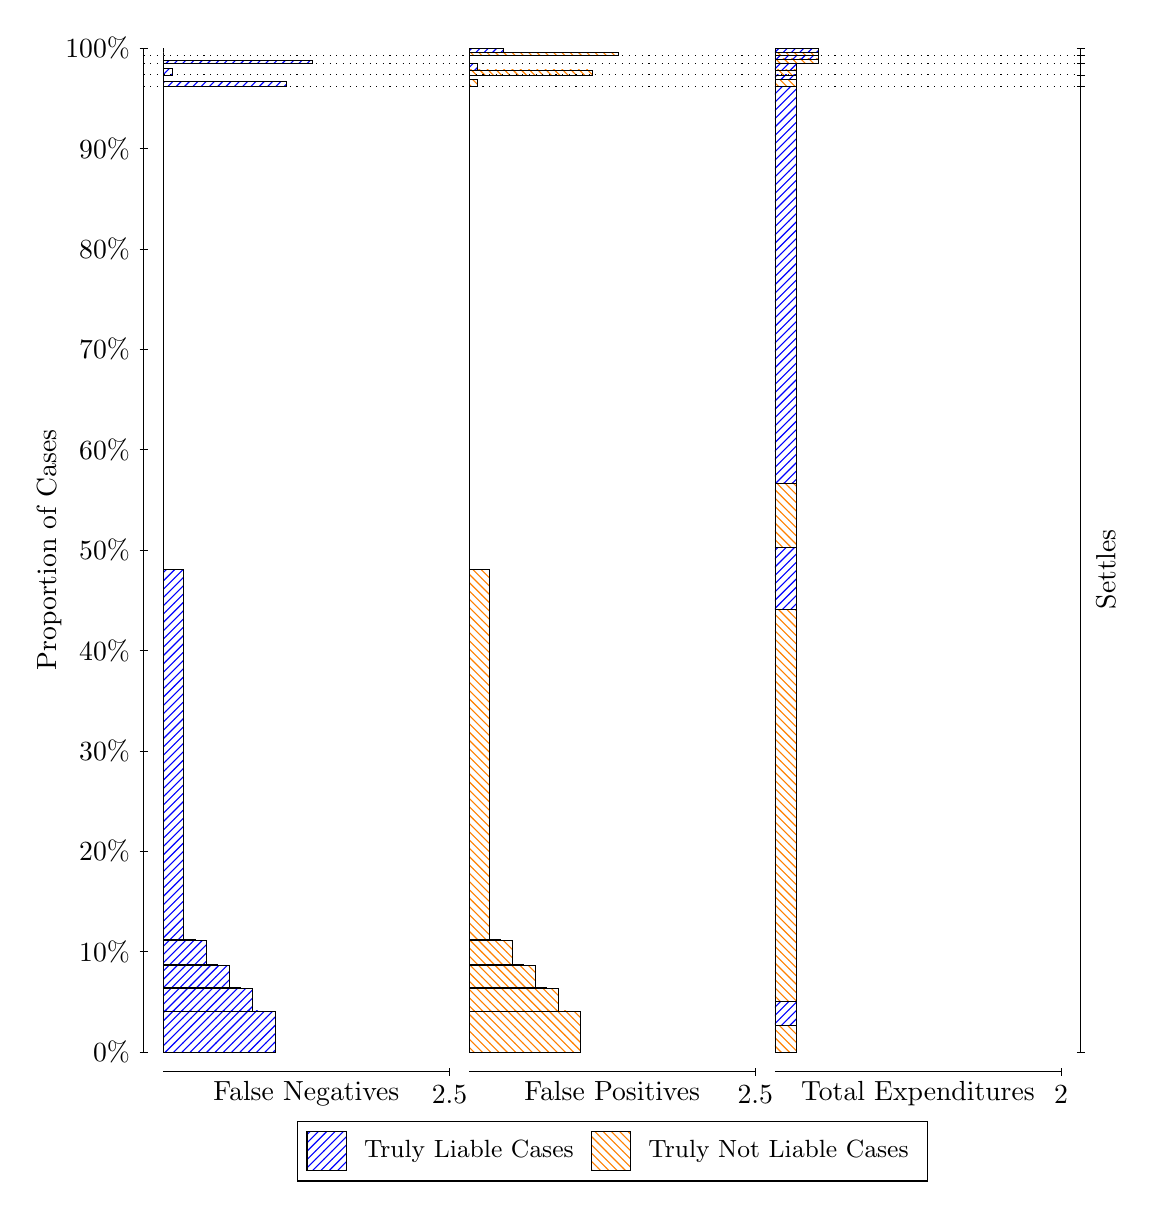
\begin{tikzpicture}
\draw[black, very thin] (1.5,1.75) -- (1.5,14.5);
\node[rotate=90, text=black, anchor=center] at (0.3, 8.125) {Proportion of Cases};
\draw[black, very thin] (1.45,1.75) -- (1.55,1.75);
\node[text=black, anchor=east] at (1.45, 1.75) {0\%};
\draw[black, very thin] (1.45,3.025) -- (1.55,3.025);
\node[text=black, anchor=east] at (1.45, 3.025) {10\%};
\draw[black, very thin] (1.45,4.3) -- (1.55,4.3);
\node[text=black, anchor=east] at (1.45, 4.3) {20\%};
\draw[black, very thin] (1.45,5.575) -- (1.55,5.575);
\node[text=black, anchor=east] at (1.45, 5.575) {30\%};
\draw[black, very thin] (1.45,6.85) -- (1.55,6.85);
\node[text=black, anchor=east] at (1.45, 6.85) {40\%};
\draw[black, very thin] (1.45,8.125) -- (1.55,8.125);
\node[text=black, anchor=east] at (1.45, 8.125) {50\%};
\draw[black, very thin] (1.45,9.4) -- (1.55,9.4);
\node[text=black, anchor=east] at (1.45, 9.4) {60\%};
\draw[black, very thin] (1.45,10.675) -- (1.55,10.675);
\node[text=black, anchor=east] at (1.45, 10.675) {70\%};
\draw[black, very thin] (1.45,11.95) -- (1.55,11.95);
\node[text=black, anchor=east] at (1.45, 11.95) {80\%};
\draw[black, very thin] (1.45,13.225) -- (1.55,13.225);
\node[text=black, anchor=east] at (1.45, 13.225) {90\%};
\draw[black, very thin] (1.45,14.5) -- (1.55,14.5);
\node[text=black, anchor=east] at (1.45, 14.5) {100\%};

\draw[black, very thin] (13.4,1.75) -- (13.4,14.5);
\draw[black, very thin] (13.35,1.75) -- (13.45,1.75);
\node[anchor=west] at (13.35, 1.75) {};
\draw[black, very thin] (13.35,14.013) -- (13.45,14.013);
\node[anchor=west] at (13.35, 14.013) {};
\draw[black, very thin] (13.35,14.159) -- (13.45,14.159);
\node[anchor=west] at (13.35, 14.159) {};
\draw[black, very thin] (13.35,14.305) -- (13.45,14.305);
\node[anchor=west] at (13.35, 14.305) {};
\draw[black, very thin] (13.35,14.403) -- (13.45,14.403);
\node[anchor=west] at (13.35, 14.403) {};
\draw[black, very thin] (13.35,14.5) -- (13.45,14.5);
\node[anchor=west] at (13.35, 14.5) {};

\draw[black, very thin, pattern color=blue, pattern=north east lines] (1.75,1.75) rectangle (3.167,2.2608);
\draw[black, very thin, pattern color=blue, pattern=north east lines] (1.75,2.2608) rectangle (3.0217,2.2708);
\draw[black, very thin, pattern color=blue, pattern=north east lines] (1.75,2.2708) rectangle (2.8763,2.5576);
\draw[black, very thin, pattern color=blue, pattern=north east lines] (1.75,2.5576) rectangle (2.731,2.5676);
\draw[black, very thin, pattern color=blue, pattern=north east lines] (1.75,2.5676) rectangle (2.5857,2.845);
\draw[black, very thin, pattern color=blue, pattern=north east lines] (1.75,2.845) rectangle (2.4403,2.8659);
\draw[black, very thin, pattern color=blue, pattern=north east lines] (1.75,2.8659) rectangle (2.295,3.1638);
\draw[black, very thin, pattern color=blue, pattern=north east lines] (1.75,3.1638) rectangle (2.1497,3.1847);
\draw[black, very thin, pattern color=blue, pattern=north east lines] (1.75,3.1847) rectangle (2.0043,7.8817);
\draw[black, very thin, pattern color=orange, pattern=north west lines] (1.75,7.8817) rectangle (1.75,14.013);
\draw[black, very thin, pattern color=blue, pattern=north east lines] (1.75,14.013) rectangle (3.3123,14.076);
\draw[black, very thin, pattern color=orange, pattern=north west lines] (1.75,14.076) rectangle (1.75,14.159);
\draw[black, very thin, pattern color=blue, pattern=north east lines] (1.75,14.159) rectangle (1.859,14.243);
\draw[black, very thin, pattern color=orange, pattern=north west lines] (1.75,14.243) rectangle (1.75,14.305);
\draw[black, very thin, pattern color=blue, pattern=north east lines] (1.75,14.305) rectangle (3.6393,14.347);
\draw[black, very thin, pattern color=orange, pattern=north west lines] (1.75,14.347) rectangle (1.75,14.403);
\draw[black, very thin, pattern color=orange, pattern=north west lines] (1.75,14.403) rectangle (1.75,14.444);
\draw[black, very thin, pattern color=blue, pattern=north east lines] (1.75,14.444) rectangle (1.75,14.5);
\draw[black, very thin, pattern color=orange, pattern=north west lines] (5.6333,1.75) rectangle (7.0503,2.2608);
\draw[black, very thin, pattern color=orange, pattern=north west lines] (5.6333,2.2608) rectangle (6.905,2.2708);
\draw[black, very thin, pattern color=orange, pattern=north west lines] (5.6333,2.2708) rectangle (6.7597,2.5576);
\draw[black, very thin, pattern color=orange, pattern=north west lines] (5.6333,2.5576) rectangle (6.6143,2.5676);
\draw[black, very thin, pattern color=orange, pattern=north west lines] (5.6333,2.5676) rectangle (6.469,2.845);
\draw[black, very thin, pattern color=orange, pattern=north west lines] (5.6333,2.845) rectangle (6.3237,2.8659);
\draw[black, very thin, pattern color=orange, pattern=north west lines] (5.6333,2.8659) rectangle (6.1783,3.1638);
\draw[black, very thin, pattern color=orange, pattern=north west lines] (5.6333,3.1638) rectangle (6.033,3.1847);
\draw[black, very thin, pattern color=orange, pattern=north west lines] (5.6333,3.1847) rectangle (5.8877,7.8818);
\draw[black, very thin, pattern color=blue, pattern=north east lines] (5.6333,7.8818) rectangle (5.6333,14.013);
\draw[black, very thin, pattern color=orange, pattern=north west lines] (5.6333,14.013) rectangle (5.7423,14.097);
\draw[black, very thin, pattern color=blue, pattern=north east lines] (5.6333,14.097) rectangle (5.6333,14.159);
\draw[black, very thin, pattern color=orange, pattern=north west lines] (5.6333,14.159) rectangle (7.1957,14.222);
\draw[black, very thin, pattern color=blue, pattern=north east lines] (5.6333,14.222) rectangle (5.7423,14.305);
\draw[black, very thin, pattern color=orange, pattern=north west lines] (5.6333,14.305) rectangle (5.6333,14.361);
\draw[black, very thin, pattern color=blue, pattern=north east lines] (5.6333,14.361) rectangle (5.6333,14.403);
\draw[black, very thin, pattern color=orange, pattern=north west lines] (5.6333,14.403) rectangle (7.5227,14.444);
\draw[black, very thin, pattern color=blue, pattern=north east lines] (5.6333,14.444) rectangle (6.0693,14.5);
\draw[black, very thin, pattern color=orange, pattern=north west lines] (9.5167,1.75) rectangle (9.7892,2.0897);
\draw[black, very thin, pattern color=blue, pattern=north east lines] (9.5167,2.0897) rectangle (9.7892,2.3964);
\draw[black, very thin, pattern color=orange, pattern=north west lines] (9.5167,2.3964) rectangle (9.7892,7.371);
\draw[black, very thin, pattern color=blue, pattern=north east lines] (9.5167,7.371) rectangle (9.7892,8.1592);
\draw[black, very thin, pattern color=orange, pattern=north west lines] (9.5167,8.1592) rectangle (9.7892,8.9768);
\draw[black, very thin, pattern color=blue, pattern=north east lines] (9.5167,8.9768) rectangle (9.7892,14.013);
\draw[black, very thin, pattern color=orange, pattern=north west lines] (9.5167,14.013) rectangle (9.7892,14.097);
\draw[black, very thin, pattern color=blue, pattern=north east lines] (9.5167,14.097) rectangle (9.7892,14.159);
\draw[black, very thin, pattern color=orange, pattern=north west lines] (9.5167,14.159) rectangle (9.7892,14.222);
\draw[black, very thin, pattern color=blue, pattern=north east lines] (9.5167,14.222) rectangle (9.7892,14.305);
\draw[black, very thin, pattern color=orange, pattern=north west lines] (9.5167,14.305) rectangle (10.062,14.361);
\draw[black, very thin, pattern color=blue, pattern=north east lines] (9.5167,14.361) rectangle (10.062,14.403);
\draw[black, very thin, pattern color=orange, pattern=north west lines] (9.5167,14.403) rectangle (10.062,14.444);
\draw[black, very thin, pattern color=blue, pattern=north east lines] (9.5167,14.444) rectangle (10.062,14.5);
\draw[black, dotted] (1.5,14.013) -- (13.4,14.013);
\draw[black, dotted] (1.5,14.159) -- (13.4,14.159);
\draw[black, dotted] (1.5,14.305) -- (13.4,14.305);
\draw[black, dotted] (1.5,14.403) -- (13.4,14.403);
\draw[black, very thin] (1.75,1.5) -- (5.3833,1.5);
\node[text=black, anchor=north] at (3.5667, 1.5) {False Negatives};
\draw[black, very thin] (5.3833,1.45) -- (5.3833,1.55);
\node[text=black, anchor=north] at (5.3833, 1.45) {2.5};

\draw[black, very thin] (5.6333,1.5) -- (9.2667,1.5);
\node[text=black, anchor=north] at (7.45, 1.5) {False Positives};
\draw[black, very thin] (9.2667,1.45) -- (9.2667,1.55);
\node[text=black, anchor=north] at (9.2667, 1.45) {2.5};

\draw[black, very thin] (9.5167,1.5) -- (13.15,1.5);
\node[text=black, anchor=north] at (11.333, 1.5) {Total Expenditures};
\draw[black, very thin] (13.15,1.45) -- (13.15,1.55);
\node[text=black, anchor=north] at (13.15, 1.45) {2};

\node[text=black, centered, rotate=90] at (13.72, 7.8817) {Settles};





\draw (7.449999999999999,1.5) node[draw=none] (baseCoordinate) {};
\begin{scope}[align=center]
        \matrix[scale=0.5, draw=black, below=0.5cm of baseCoordinate, nodes={draw}, column sep=0.1cm]{
            \node[rectangle, draw, minimum width=0.5cm, minimum height=0.5cm, pattern color=blue, pattern=north east lines] {}; &
            \node[draw=none, font=\small, text=black] (B) {Truly Liable Cases}; &
            \node[rectangle, draw, minimum width=0.5cm, minimum height=0.5cm, pattern color=orange, pattern=north west lines] {}; &
            \node[draw=none, font=\small, text=black] (B) {Truly Not Liable Cases}; \\
            };
\end{scope}

\end{tikzpicture}
\end{document}